\chapter{研究现状概述}
随着移动通信技术和个人设备的迅速发展,移动直播的应用呈现井喷式发展。据思科公司的数据预测,未来3年网络直播会占据总视频流量的13\%。移动直播用户数量大幅度增长的同时,用户对于直播服务质量的要求也随之提高。

传统直播能够将视频通过网络分发给大量的用户,为广大用户提供视频服务。但传统直播的不足之处在于要求为主播端预留专线带宽,且端到端的时延较大。在大量用户渴望成为直播内容贡献者的今天,要求每个主播都拥有专线带宽并不可行;而且传统直播的高时延无法满足观众对于直播互动性的要求。


\section{直播传输优化研究现状}
\subsection{直播发展现状}
传统直播的系统架构和交互直播基本相同,传统直播也由三部分组成,视频源端到源服务器,源服务器到CDN边缘服务器,CDN边缘服务器到观众。但传统直播的视频源端到源服务器的链路一般为预先分配的专有链路,所以传统直播研究的重点集中在源服务器到观众端的部分。从源服务器到观众端主要有两种分发架构,CDN网络~\cite{mukerjee2015practical}和P2P网络~\cite{liao2006anysee}~\cite{hei2007inferring}~\cite{magharei2007mesh}。CDN网络分发和P2P网络分发各有优缺点,CDN网络分发时会根据网络负载去选择负载轻的服务器,根据用户的带宽去选择合适的码率。当网络中服务器负载不高时,CDN网络分发能给终端用户提供较高的体验质量。但为了保证用户的体验质量,CDN网络需要保证网络各服务节点负载不高,因此需要配置相当数量的服务器,运营成本较高。相比较而言,P2P网络具有高度可扩展性,对服务器的负载要求较少,然而P2P这种去中心化的合作方式大规模应用的话会有一些缺点,比如,用户接收到的视频质量低,节点之间负载不均衡,无法进行网络监管等问题。

\begin{figure}[h]% use float package if you want it here
  \centering
  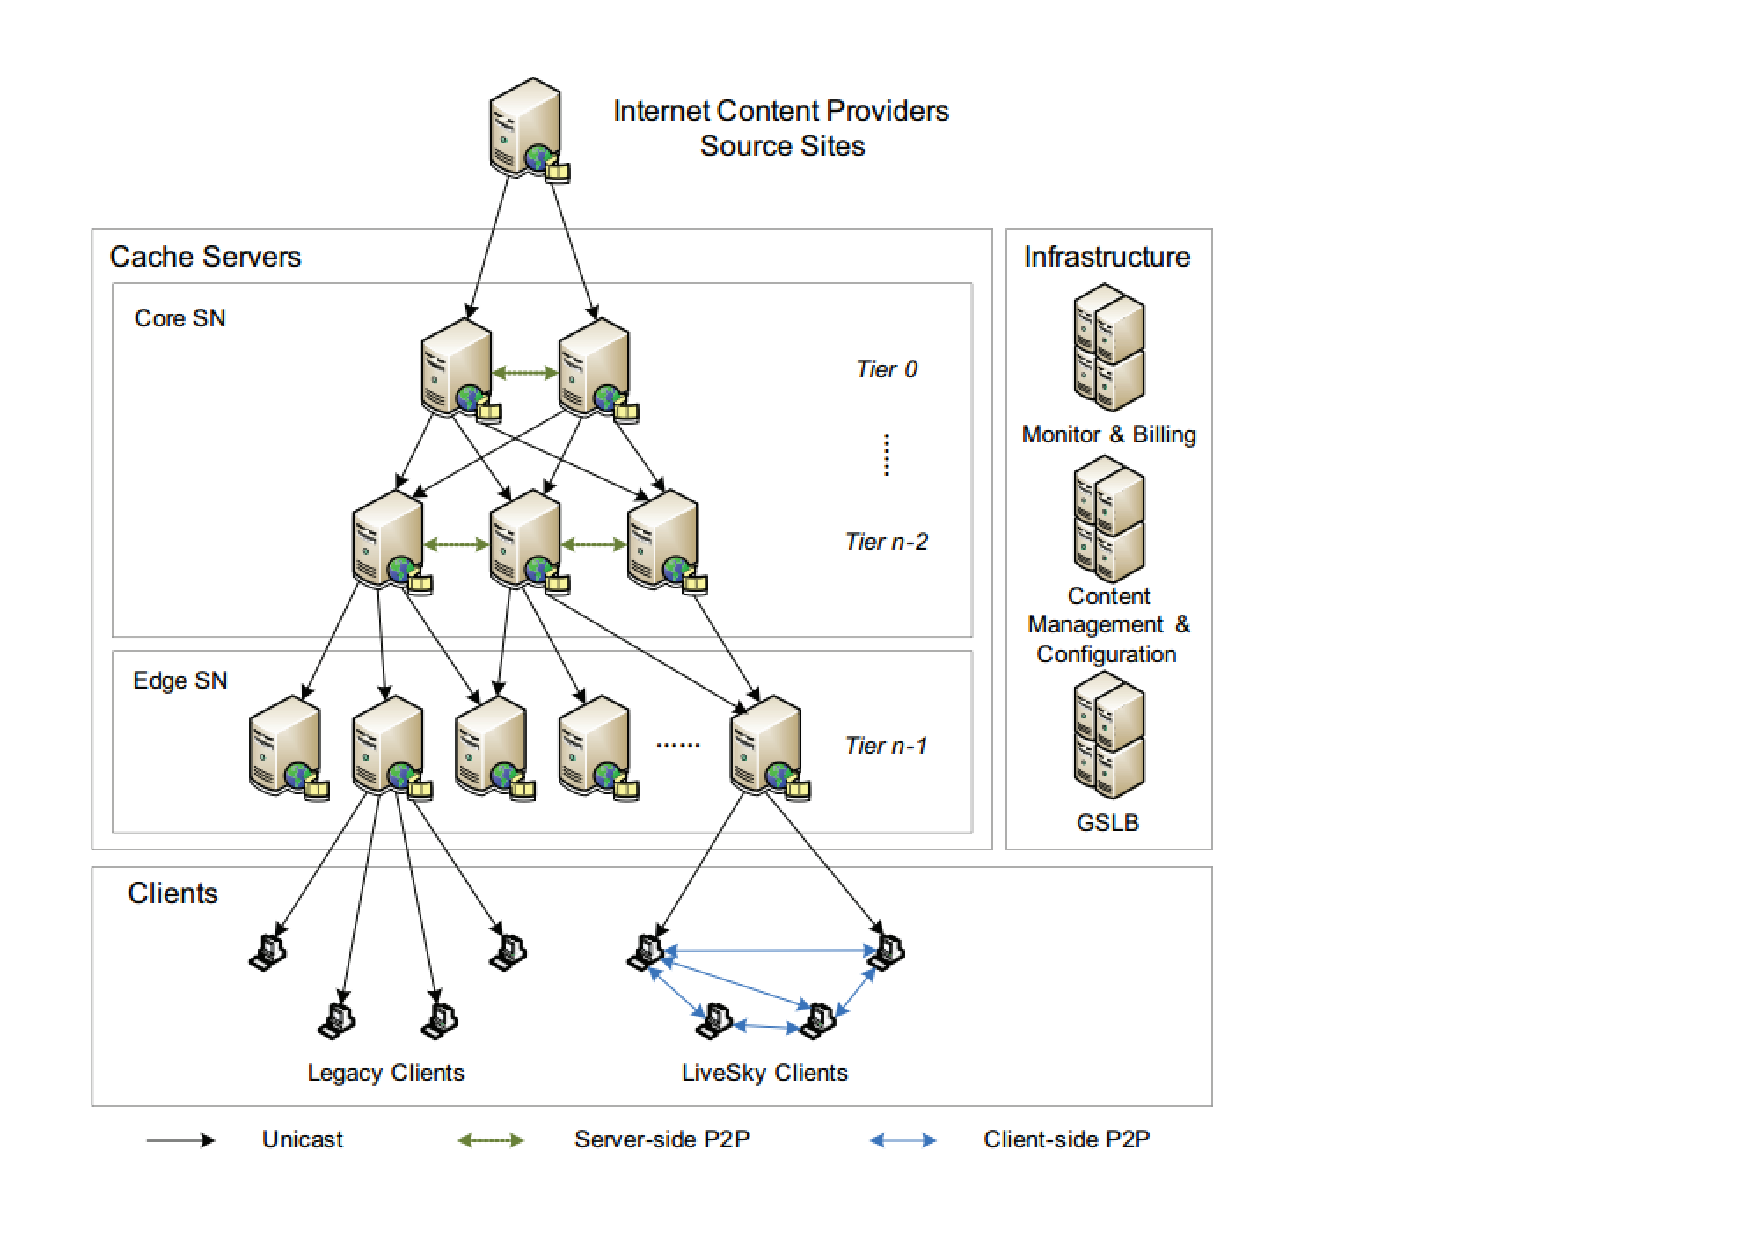
\includegraphics[width=0.9\textwidth]{livesky}
  \caption{LiveSky系统架构图~\cite{yin2009design}}
  \label{fig:livesky}
\end{figure}

Yin等学者~\cite{yin2009design}提出了P2P网络和CDN网络混合分发的LiveSky架构,并在实际中部署,LiveSky的系统图如图~\ref{fig:livesky}所示。针对P2P和CDN的联合架构,Yin等人设计了一个分段阈值式的资源动态分配机制,在用户规模增大的情况下依然能提供良好的视频观看体验。同时他们利用CDN的边缘服务器和重定向机制去解决P2P系统的不足,使得采用NAT地址转换的用户也可以完成上传,保证对现有网络而言的公平性。

学术界目前关于个人交互直播的研究多数还只是着眼于分析直播用户的行为,以及对交互直播系统框架的解剖。Zhang等学者~\cite{zhang2015crowdsourced}通过爬取Twitch网站~\cite{Twitch}提供的数据,抓取本地主播端的流量勾勒出了交互直播的内部架构;另外,通过对Twitch网站数据两个月的抓取,Zhang等发现用户的观看行为基本由重大事件和主播决定。另外,观众端感受到的时延会严重影响观看的交互体验。Twitch将直播视频分发和信息发送分开来实现,因此直播消息的时延很短,视频时延很长,两者之间差别很大。另外,Zhang等学者改变主播端的带宽容量发现,主播端的带宽容量会明显影响直播视频播放的流畅性。

Meerkat和Periscope是另外两个国外主流的移动直播应用,主要部署在移动端。Matti等作者重点研究了Periscope应用的用户体验质量~\cite{siekkinen2016first},主要是播放流畅性,延迟和能量消耗等相关因素。Periscope的接口信息是通过HTTPS加密的方式传播的,Matti等人通过建立透明代理的方式去截取Periscope应用接口的信息。并且Periscope的接口并不直接给出平台的总用户数信息,只提供邻近地区的用户数,Matti等人通过深度挖掘每个地区用户量的方法去组合获取实时的总用户量。另外,Periscope主播用户的粉丝数呈现长尾分布,主播用户的粉丝数会影响主播用户的积极性,粉丝数少的主播直播时长会相应的变短。

直播应用一般会给每个主播分配一个独一无二的ID,Wang等作者利用这个特性~\cite{wang2016anatomy},以高频率的轮询算法随机观看直播,去计算Meerkat~\cite{Meerkat}和Periscope的用户数和主播数。另外,Wang等人发现Periscope直播平台为了增加系统的可拓展性,在用户数小于100时,直接使用RTMP协议进行分发,当用户数超过100时,多出来的用户通过HTTP协议进行直播视频分发。Wang等人对两种协议情况下主播端到用户端的每一段引入的时延进行了分析,发现使用HTTP协议分发视频,相比于使用RTMP协议直接获取视频,引入了切块时延和用户请求延时。 另外,使用HTTP协议进行视频分发时,用户端的缓存策略一般比较保守,缓存时间较长,从而导致较大的缓存时延。

关于优化直播传输质量的研究很少,但通过优化主播端的传输质量来优化用户体验质量的研究更加稀少。

\subsection{直播协议研究现状}
在众多视频传输协议中,HTTP协议凭借广泛部署的CDN网络以及易穿透防火墙,服务器代码开源等特性,逐渐成为视频点播领域的主流协议~\cite{li2013two}。现在的HTTP协议在视频方面主要有APPLE的HLS(HTTP Live Streaming)协议~\cite{Apple}和DASH(Dynamic Adaptive Streaming over HTTP)协议~\cite{stockhammer2011dynamic}~\cite{sodagar2011mpeg},两者的原理基本相同。HTTP协议都会对视频进行切块操作,将一个完整视频切为许多4-10s的视频块,视频块是传输和处理的基本单元。HTTP协议的延时较高,主要是因为只有当一个视频块完整的产生后,CDN端才开始分发,用户端才能开始播放,所以不可避免的至少有一个视频块的延时,称为切片时延。由于切片时延的存在,且切片时延一般为数秒的量级,HTTP协议的延时一般都较大,因此HTTP协议在直播领域的应用较少。

针对HTTP协议的切块时延,一个比较直接的解决方案是减少视频块的时长,减到直播情景可以接受的时间长度,减小由于视频切块带来的时延。但是若直接减少视频块的时长,会导致HTTP请求数的倍速增长,使得HTTP服务器的负载过大。客户端发起的HTTP请求数和视频块的时长成反比,比如,对于一个60秒的直播视频,如果每个视频块是4秒,总的请求响应数目为15;但当我们把视频块的时长缩短为1秒时,总的请求响应数目会增长为60。因为每个HTTP请求和响应都会有头部报文,倍数增长的请求响应给服务器和网络设备带来了额外的处理开销,这对HTTP视频流的可扩展性造成了极大的影响。

\begin{figure}[htb]
  \centering%
  \begin{subfigure}{0.45\textwidth}
    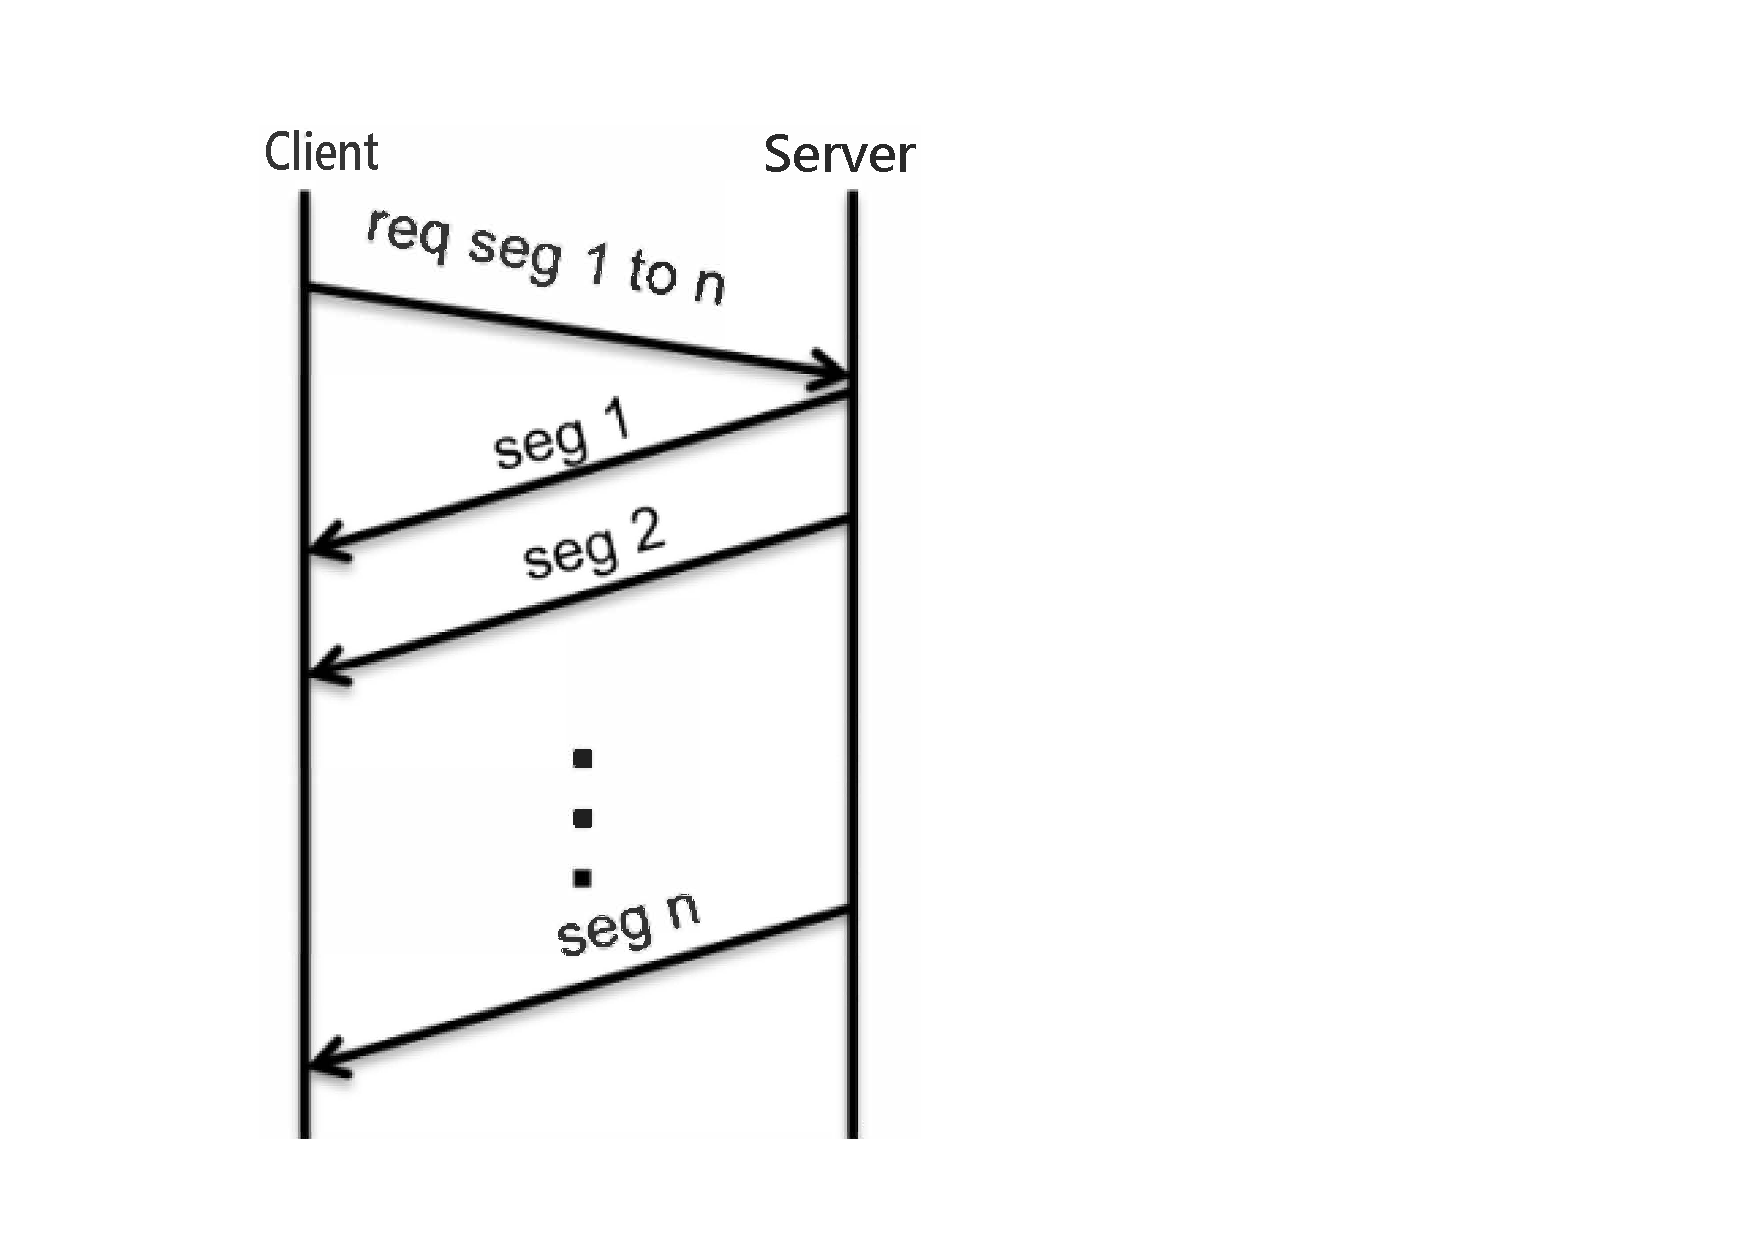
\includegraphics[width=\textwidth]{all-push}
    \caption{一次推送全部内容}
    \label{fig:all_push}
  \end{subfigure}%
  \hfill
  \begin{subfigure}{0.45\textwidth}
    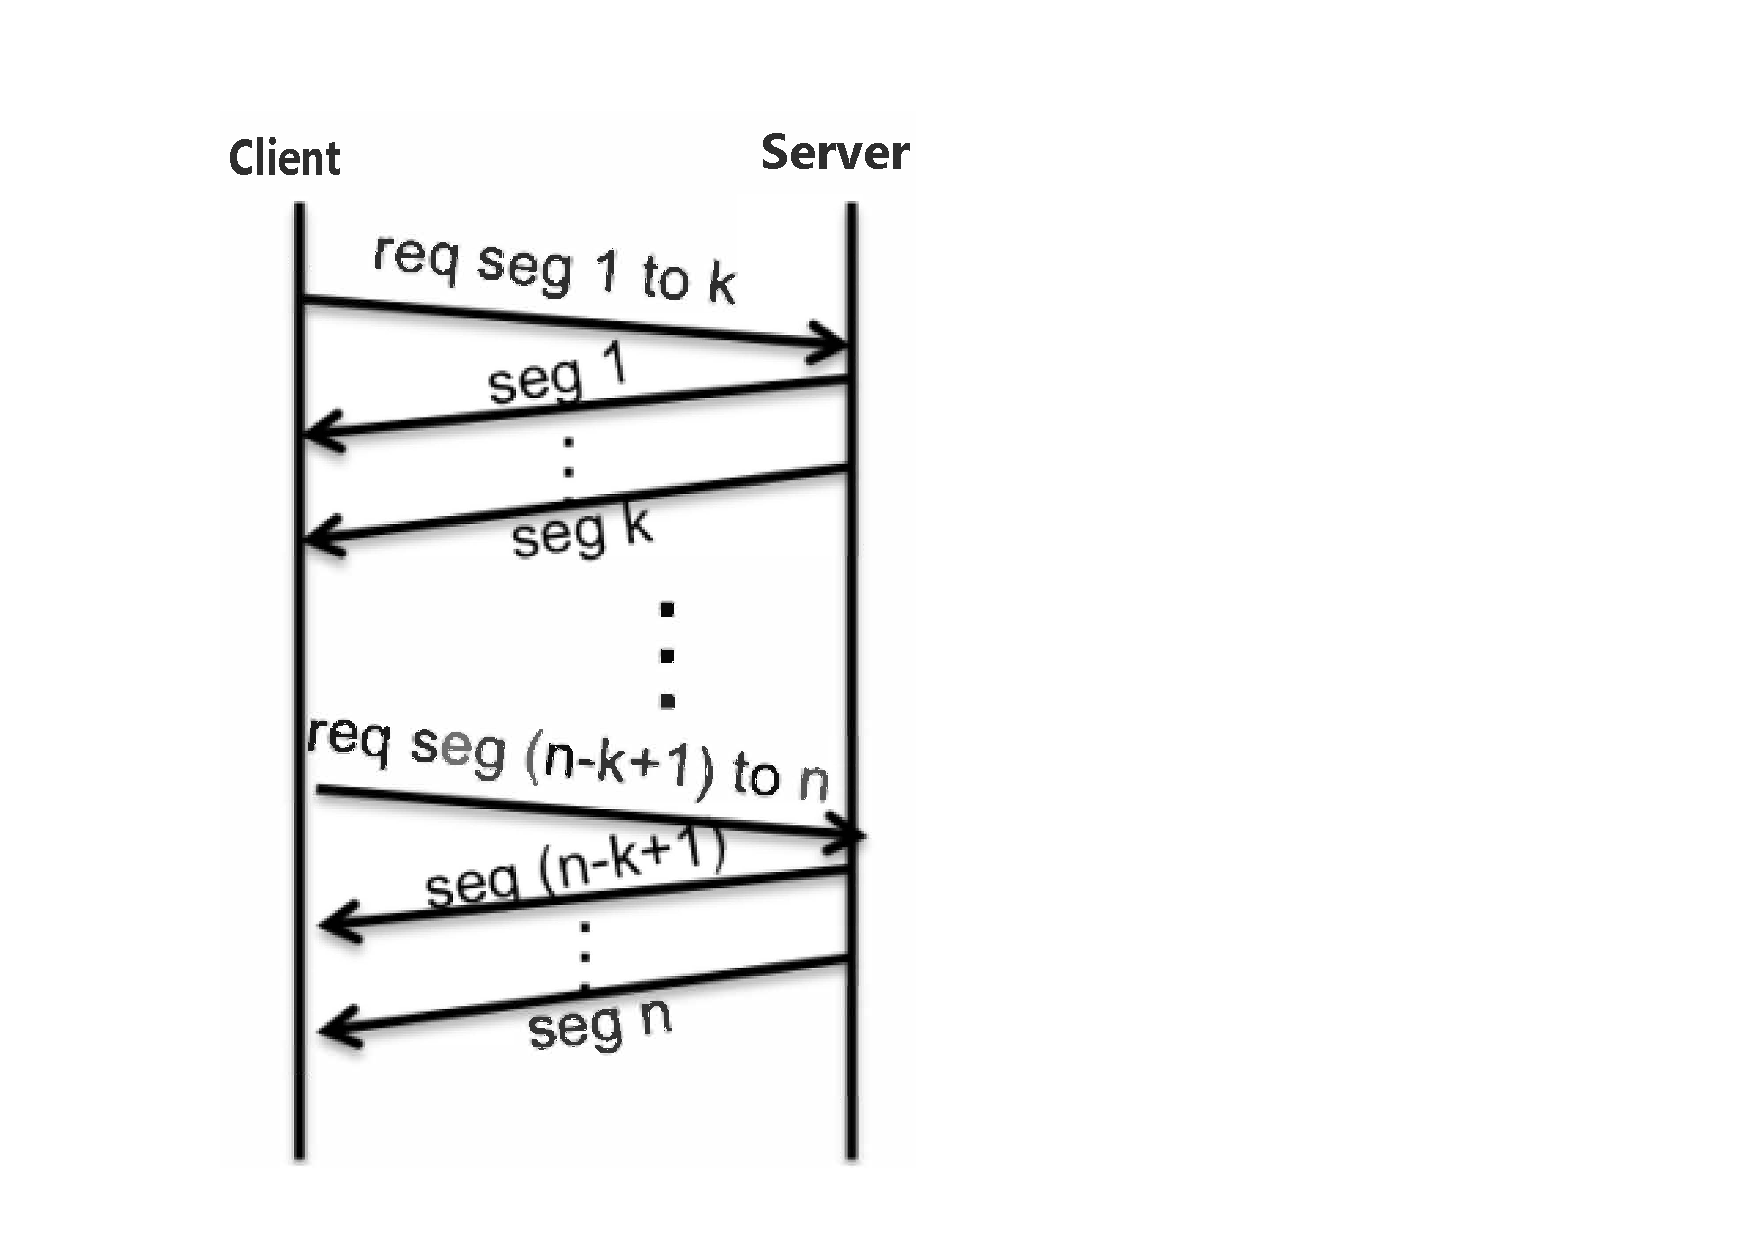
\includegraphics[width=\textwidth]{k-push}
    \caption{一次推送多个内容}
    \label{fig:k_push}
  \end{subfigure}
  \caption{HTTP协议2.0版本的新特性~\cite{wei2014low}}
  \label{fig:push}
\end{figure}

学术界有一些研究尝试将HTTP技术应用到直播中来,研究如何解决HTTP协议的切块延时过长问题。HTTP协议2.0版本引入的服务器推流特性允许服务器直接将资源推流到客户端,不需要客户端去明示的请求资源,这个特性极有可能打破视频块大小和请求数之间的反比关系。Wei等学者便尝试利用HTTP协议2.0的推流特性去减少切块时延~\cite{wei2014low},因为HTTP协议2.0并不是专门的视频传输协议,因此Wei等人提出了一个定制的视频推流策略。利用HTTP服务器推流减少时延的主要思路是尽可能减少视频块的时长直到满足时延要求。推流策略需要解决的问题有两个方面:推哪些内容和什么时候推。文章给出了两种策略,一次请求推送全部内容和一次请求推送多个内容,如图~\ref{fig:push}。文章通过大量的实验说明,使用服务端推流的特性,直播的时延可以大大的降低。

HTTP协议的分块传输编码机制也被用来减少HTTP协议中端到端的时延~\cite{swaminathan2011low}。Swaminathan等学者在文章中提供了两种减少端到端时延的方案,分别是服务器等待策略和分块编码策略。服务器等待的策略和原来的视频块策略相比,只做了些微的修改。最根本的改变是客户端请求正在生成的新视频块,而不是已经生成的视频块。为了达到这一目的,客户端请求描述文件中最新视频块的后面一个视频块。因为请求的视频块尚未生成,所以服务器在收到请求后一直处于等待状态,直到视频块生成为止。服务器等待的策略减少了将近一个视频块的时延,但这个优化的程度还远远不够。为了进一步优化端到端时延,Swaminathan等人进一步提出了分块编码策略。和服务器等待策略相同,分块编码策略也总是请求后面一个视频块。分块编码策略中,服务器端将视频块切分为均匀的多个视频片段,收到客户端的请求后,将编码完成的视频片段先发送出去,之后陆续将剩余的视频片段发送出去。不同于最简单的HTTP协议,HTTP分块编码允许在服务器端维护一个HTTP长连接,客户端只需要一次请求,就可以接收数次响应消息。利用分块编码,同时将每个视频块的时长增大,分块编码达到了减少时延的效果,将时延降低为1~2个视频片段的时长。

Bouzakaria等人利用GDR(Gradual Decoding Refresh)~\cite{hannuksela2003random}技术去编码,将直播视频编码成ISO基本媒体文件格式,并在传输层使用分块编码传输策略去减少HTTP协议的时延~\cite{bouzakaria2014overhead}。GDR技术是相对于用完整的一个视频帧来刷新的技术而言的。传统的完整帧刷新编码技术有一定的缺点,关键帧相对于其余的帧体积过大,容易对网络造成冲击,导致网络抖动。而GDR技术将关键帧分散到几个非关键帧中,缓解了对网络带来的冲击。Bouzakaria等人采用和Swanubathan类似的思路,改造了DASH传输协议的MPD文件,在原有MPD文件中添加了一个字段:有效时间偏差。有效时间偏差代表了新的视频块可以请求的时间,即使新的视频块可能只产生了一部分片段。有效时间偏差字段使得客户端提前得知有新的视频块产生,并提前发起请求,有效减少了HTTP协议的延迟。

上述研究都一定程度上解决了HTTP协议的低时延问题,但目前商业化平台应用仍然只在视频分发时使用HTTP协议,因此我们研究的重点依然集中在主播端使用较多的RTMP协议。

\subsection{码率自适应研究现状}
关于码率自适应研究的文章很多,其中大部分都集中在点播领域~\cite{mao2017neural}~\cite{akhshabi2011experimental}~\cite{petrangeli2016qoe}。点播领域的码率自适应算法可以分为三类:基于带宽的,基于缓存的,以及两者的结合。

FESTIVE~\cite{jiang2014improving}就是典型的基于带宽的码率自适应算法。FESTIVE通过测量现有的商业级播放器,包括Netflix,Adobe OSMF等,发现当多个动态码率播放器共享同一链路时,会出现带宽分配不均匀的问题。另外,高码率和码率的稳定性在动态码率情况下也是应该考虑的重点。针对这三个性能指标,FESTIVE提出了一整套的解决方案。FESTIVE采用随机调度视频块的方式去减缓其他播放器下载视频占用带宽带来的带宽探测误差,从而尽量避免带宽分配的不均匀;用状态转移的方式去选择码率,拟合码率和预估带宽之间的偏差;码率延迟更新策略,以达到高码率和码率稳定性之间的平衡。

大多数码率自适应算法都是基于带宽去选择码率~\cite{li2014probe}~\cite{akhshabi2012happens},但是对于无线网络环境,尤其是在移动设备的情况下,带宽变化剧烈,很难去精确的预测带宽。Huang等人~\cite{huang2015buffer}首次创新性的提出了基于缓存的数据量去选择码率的算法。视频播放一般可以划分为两个阶段:启动阶段和稳定阶段。视频开始播放时,缓存的数据先从零开始积累到一个阈值,之后边下边播,缓存进入稳定阶段。基于缓存选择码率的算法基于一个想法:当缓存数据量较大时,用户端可以选择较高点的码率,提高码率的收益;如果缓存数据量较小,那用户端应该保守一些,选择较低点的码率,以保证不卡顿流畅播放。在开始阶段,缓存相关信息量较少,此时利用带宽预测的信息选择码率是很有必要的;但一旦进入稳定阶段,缓存数据量相关的信息充足时,只根据缓存去选择码率也可以性能很好。

Yin等学者~\cite{yin2015control}利用模型预测控制理论(MPC)来优化码率选择。MPC尝试预测未来一段时间的网络环境,模拟未来一段时间的系统状态,遍历求得一段时间的最优解决方案,然后只采用下一时隙的解决方案,循环往复。MPC将之前基于码率和基于缓存的方案结合起来,在优化时将码率和缓存同时纳入了优化空间,MPC的优化空间如图所示。另外,求一段时间内的最优方案有更大可能会优于某一时刻的最优。码率遍历选择的算法由于其高时间复杂度在实际运行中会面临问题,Yin等人提出了基于查询缓存结果的FastMPC算法,相对现有的所有算法提高了10\%-15\%的平均用户体验质量。

点播和直播领域的码率自适应主要有两点不同。第一个不同点是时间粒度,点播动态码率的粒度为一个视频块,而一个视频块持续4-10s秒时间;直播码率变化的粒度为一个GoP或者更小,一个GoP通常为2秒左右。第二个不同点是缓存队列的大小,点播时通常会缓存数十秒以防止播放的卡顿;而直播时缓存最少不超过1秒,否则会增加端到端的时延。

学术界也有一些关于直播如何使用码率自适应技术的研究。Pires等人~\cite{pires2014dash}通过对Twitch平台用户规模以及用户行为的研究,提出可以应用码率自适应技术分发直播流。直播的流程如图~\ref{fig:architecture}所示,如果想要应用码率自适应技术进行视频分发,需要在源服务器处进行转码,将主播端上传的单一码率视频转码为多个码率,之后用户选择自己适合的码率。Twitch平台上并发的主播数量很多,对所有主播直播的视频进行转码会需要消耗大量的计算资源。文章考虑主播的观众数,转码带来总的用户体验质量的提升以及资源消耗等因素的折中,选择部分主播进行转码操作。

Bouzakaria等学者~\cite{bouzakaria2014overhead}尝试用动态码率自适应技术去实现超低时延的直播。动态码率自适应技术的时延主要有几个部分构成:切块时延,下载视频块的时间,以及用户端的缓存时长。如果将视频块切成更小的数据块在网络中传输,切块时延也会减小为小视频块的时长。之前的CDN和播放器都是在接收到一个完整的视频块之后,才开始转发以及播放。为了进一步减少时延,Bouzakaria等学者修改了视频信息描述文件,并且使用HTTP协议的分块传输编码,一旦接收到一个视频块的一段,就可以开始分发和播放,将原有的一个视频块的时延减少为一段的时延。

\begin{figure}[h]% use float package if you want it here
  \centering
  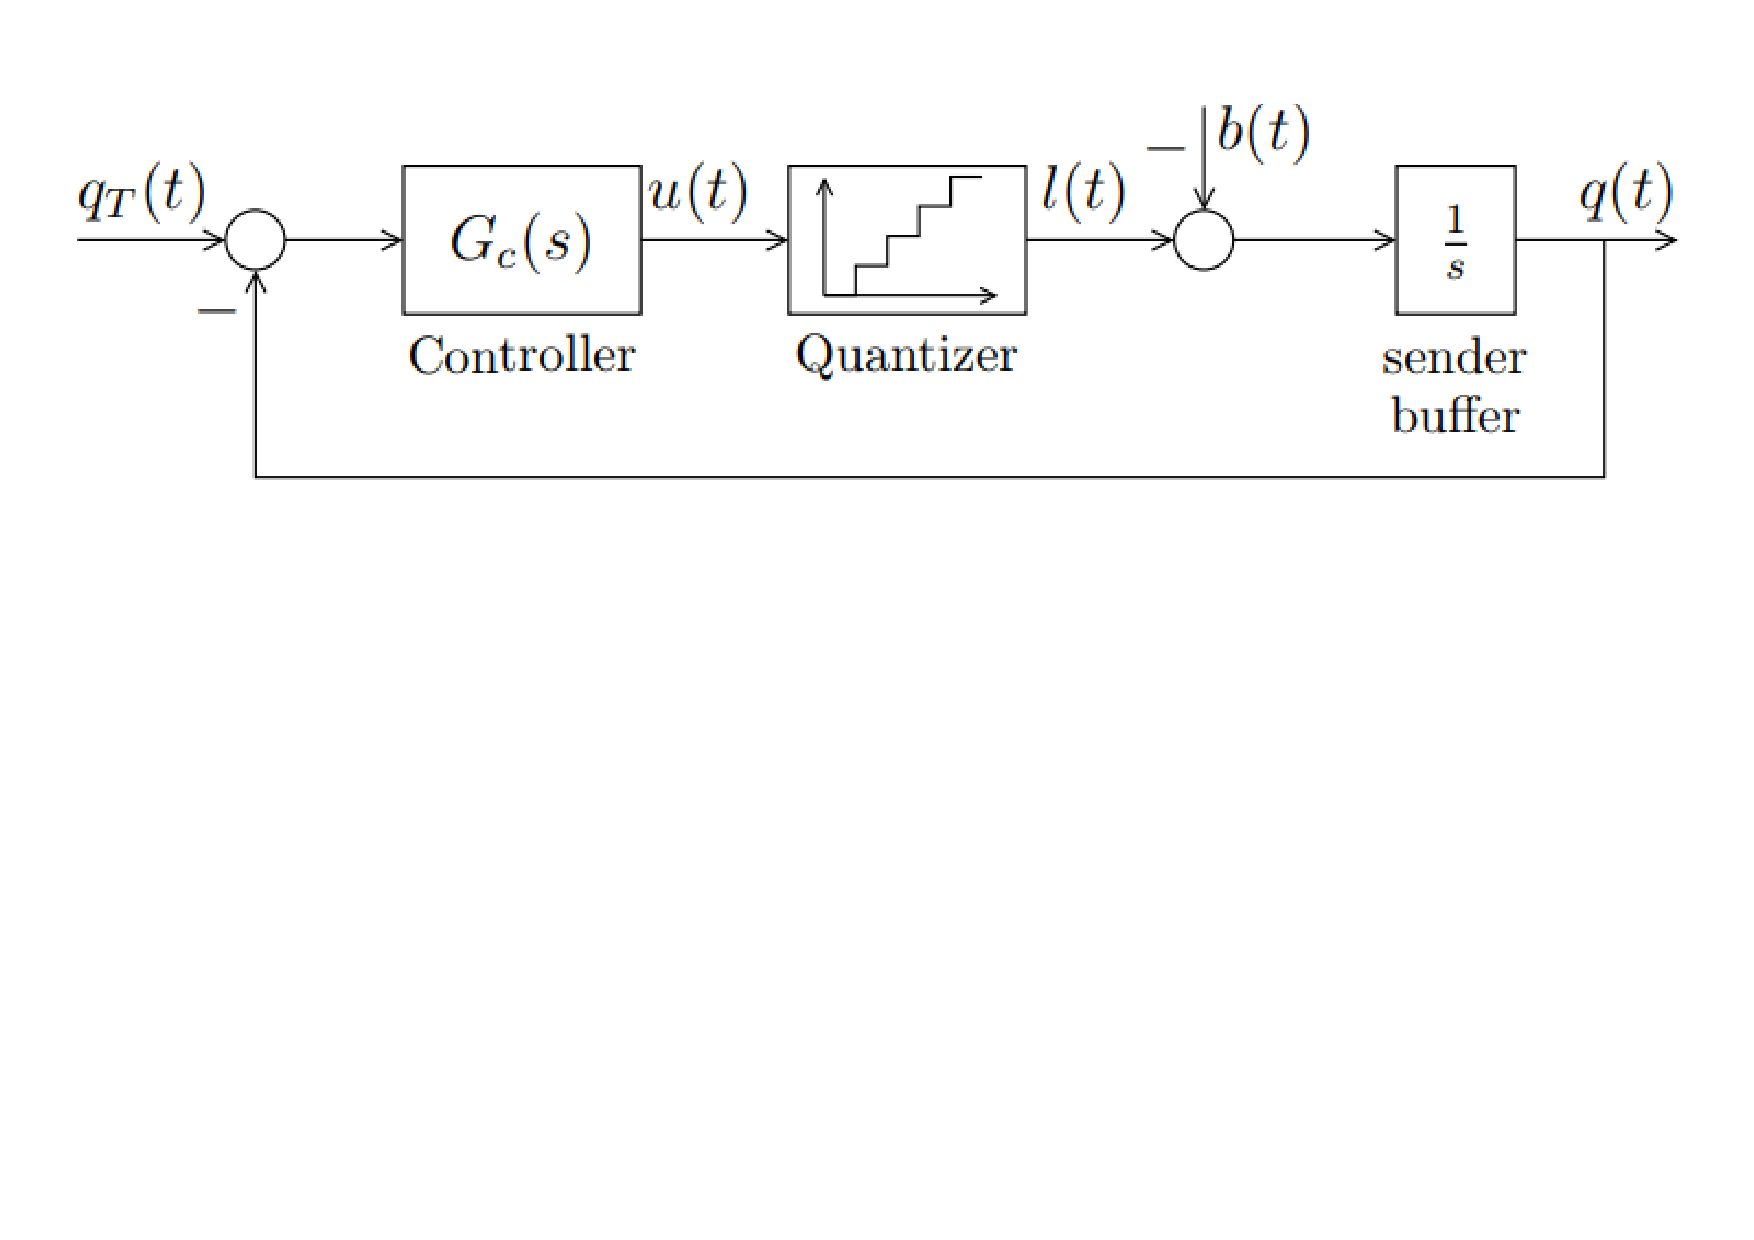
\includegraphics[width=0.9\textwidth]{feedback_control}
  \caption{反馈控制理论~\cite{de2011feedback}}
  \label{fig:feedback_control}
\end{figure}

De等人~\cite{de2011feedback}用反馈控制理论去选择最优码率。不同于之前的启发式算法,反馈控制理论可以得到一个可预测的系统状况,更方便下一时隙的码率选择。控制器工作流程如下图~\ref{fig:feedback_control}:发送端的缓存大小作为输入,$q_T$是发送端缓存的阈值。控制器的激活部分,以发送端现在的缓存大小和阈值$q_T$的差作为输入,输出控制信号。输出的控制信号经过量化,选择最大的小于量化后的值的码率,即为最后所选择的码率。

上述关于在直播中使用码率自适应技术的研究多数关注于如何大规模部署码率自适应技术,以及超低时延的码率自适应技术,De等人的研究虽然关注于如何选择码率最优,但是研究的是点对点的直播,且端到端的延时较大。总体来说关于如何优化直播应用主播端的传输质量的研究很少,所以我们的研究也具有一定的挑战性。

\subsection{交互直播的性能要求}
点播情景下对于系统的性能要求一般是三点:高码率,敏捷平滑的码率切换以及低卡顿率。但主播端不同于点播客户端的根本一点在于,点播的客户端是被动接收请求的视频,而主播端负责将摄像头编码产生的视频推送出去。网络状况不好时,点播的客户端接收视频会受影响,导致视频播放出现卡顿;但对于主播端来说,网络状况不好,视频的上传会受到影响,从而导致视频帧从产生到到达用户端的时延过长,用户观看直播的过程中出现黑屏。经过上述分析,移动网络带宽不稳定的状况下,观众和主播间的高交互性要求对直播的主播端提出了如下的性能要求。
\begin{itemize}
  \item 尽可能高的视频质量。视频质量的优劣,和视频的码率,每秒的帧率,以及分辨率都息息相关。在帧率和分辨率固定的情况下,主播端应上传尽可能高的码率到源服务器。源头的码率高,下游的用户才有可能接收到清晰的视频,得到满意的用户体验质量。
  \item 敏捷平滑的码率自适应。交互直播一般都处于移动网络环境下,网络带宽十分不稳定。主播端的码率变化必须足够灵活敏捷,能够快速响应无线网络中的带宽波动。同时,如果应用码率自适应技术,码率的平滑切换也是一个重要的指标。码率的平滑切换要求码率的切换幅度尽量小,切换次数尽量少。
  \item 直播的及时性。为了保证直播的高交互性和用户的高参与度,必须最小化主播端和用户之间的时延,或者限制住最大的时延。端到端的时延要求反映在主播端,则对应于帧发送的时间和帧产生的时间差要满足一定的约束。
\end{itemize}

RTMP协议将视频帧作为基本的传输单位,码率的转换和调整都足够灵活,因此有可能能够满足上述三个性能要求。比如,它在主播端提供了大量可供调节的参数接口,可以调整视频质量,包括每秒的帧率,视频队列的大小,还有丢帧策略的相关参数。理论上来说,合适的丢帧策略需要在视频质量和及时性两者之间维持一个动态均衡~\cite{krasic2003quality}~\cite{singh2004dynamic}~\cite{huang2003adaptive}~\cite{fouladi2018salsify}。直播情境下RTMP协议依然是主旋律。然而,在下章我们会给出,现在开源的RTMP实现以及商业级应用都存在严重的质量问题。

\section{本章小结}
本章首先以传统直播和交互直播的两大关键不同点作为切入点,个人直播相对于传统直播而言个人直播对传输技术提出了更高的挑战,因为个人直播的网络环境一般为无线网络,且用户和主播的强交互性对端到端的时延的要求较高。之后我们给出了现在的较为主流的直播传输框架,在主播端上传时使用RTMP协议,分发时使用HTTP协议借助CDN网络完成。

本章从三个角度来介绍直播传输协议的演变过程,直播框架,直播协议和自适应码率技术。传统直播一般使用P2P网络或者CDN网络来进行分发,还有用两种网络混合的架构来进行分发,交互直播架构的研究目前还只是停留在通过测量去发现现有直播的架构的地步。直播协议方面,RTMP协议因其较低的端到端时延而在直播应用中使用较多。HTTP协议因为至少一个视频块时长的时延而较少应用在直播中,但目前也有一些研究集中在减少HTTP协议的时延方面。码率自适应技术目前较多的研究集中在点播领域,直播方面目前的研究只涵盖了点对点的直播,多用户情景的研究较少。

另外,本章给出了交互直播的三点性能要求,高码率,少切换以及端到端的时延。后续的几章内容主要通过测量发现直播系统中的问题,并尝试设计出一套相应的解决方案。
